\documentclass[tikz,border=8pt]{standalone}
\usepackage[T1]{fontenc}
\usepackage[utf8]{inputenc}
\usepackage{lmodern}
\usepackage{xcolor}
\usetikzlibrary{arrows.meta,positioning,fit,shapes.misc}

\definecolor{astblue}{HTML}{DCEEFF}
\definecolor{astgreen}{HTML}{DFF5E1}
\definecolor{astyellow}{HTML}{FFF3CC}
\definecolor{astpink}{HTML}{FBE1EA}
\definecolor{astgray}{HTML}{F4F4F4}
\definecolor{astline}{HTML}{5A6B7A}

\tikzset{
  box/.style={
    draw=astline,
    rounded corners=3pt,
    thick,
    align=left,
    font=\sffamily\small,
    text width=4.6cm,
    inner sep=6pt
  },
  smallbox/.style={
    draw=astline,
    rounded corners=3pt,
    thick,
    align=left,
    font=\sffamily\small,
    text width=3.8cm,
    inner sep=6pt
  },
  title/.style={
    font=\sffamily\bfseries\Large,
    text=black
  },
  arrow/.style={
    -{Latex[length=3mm,width=2mm]},
    thick,
    draw=astline
  },
  note/.style={
    font=\sffamily\footnotesize,
    text=black!75,
    align=left
  }
}

\begin{document}
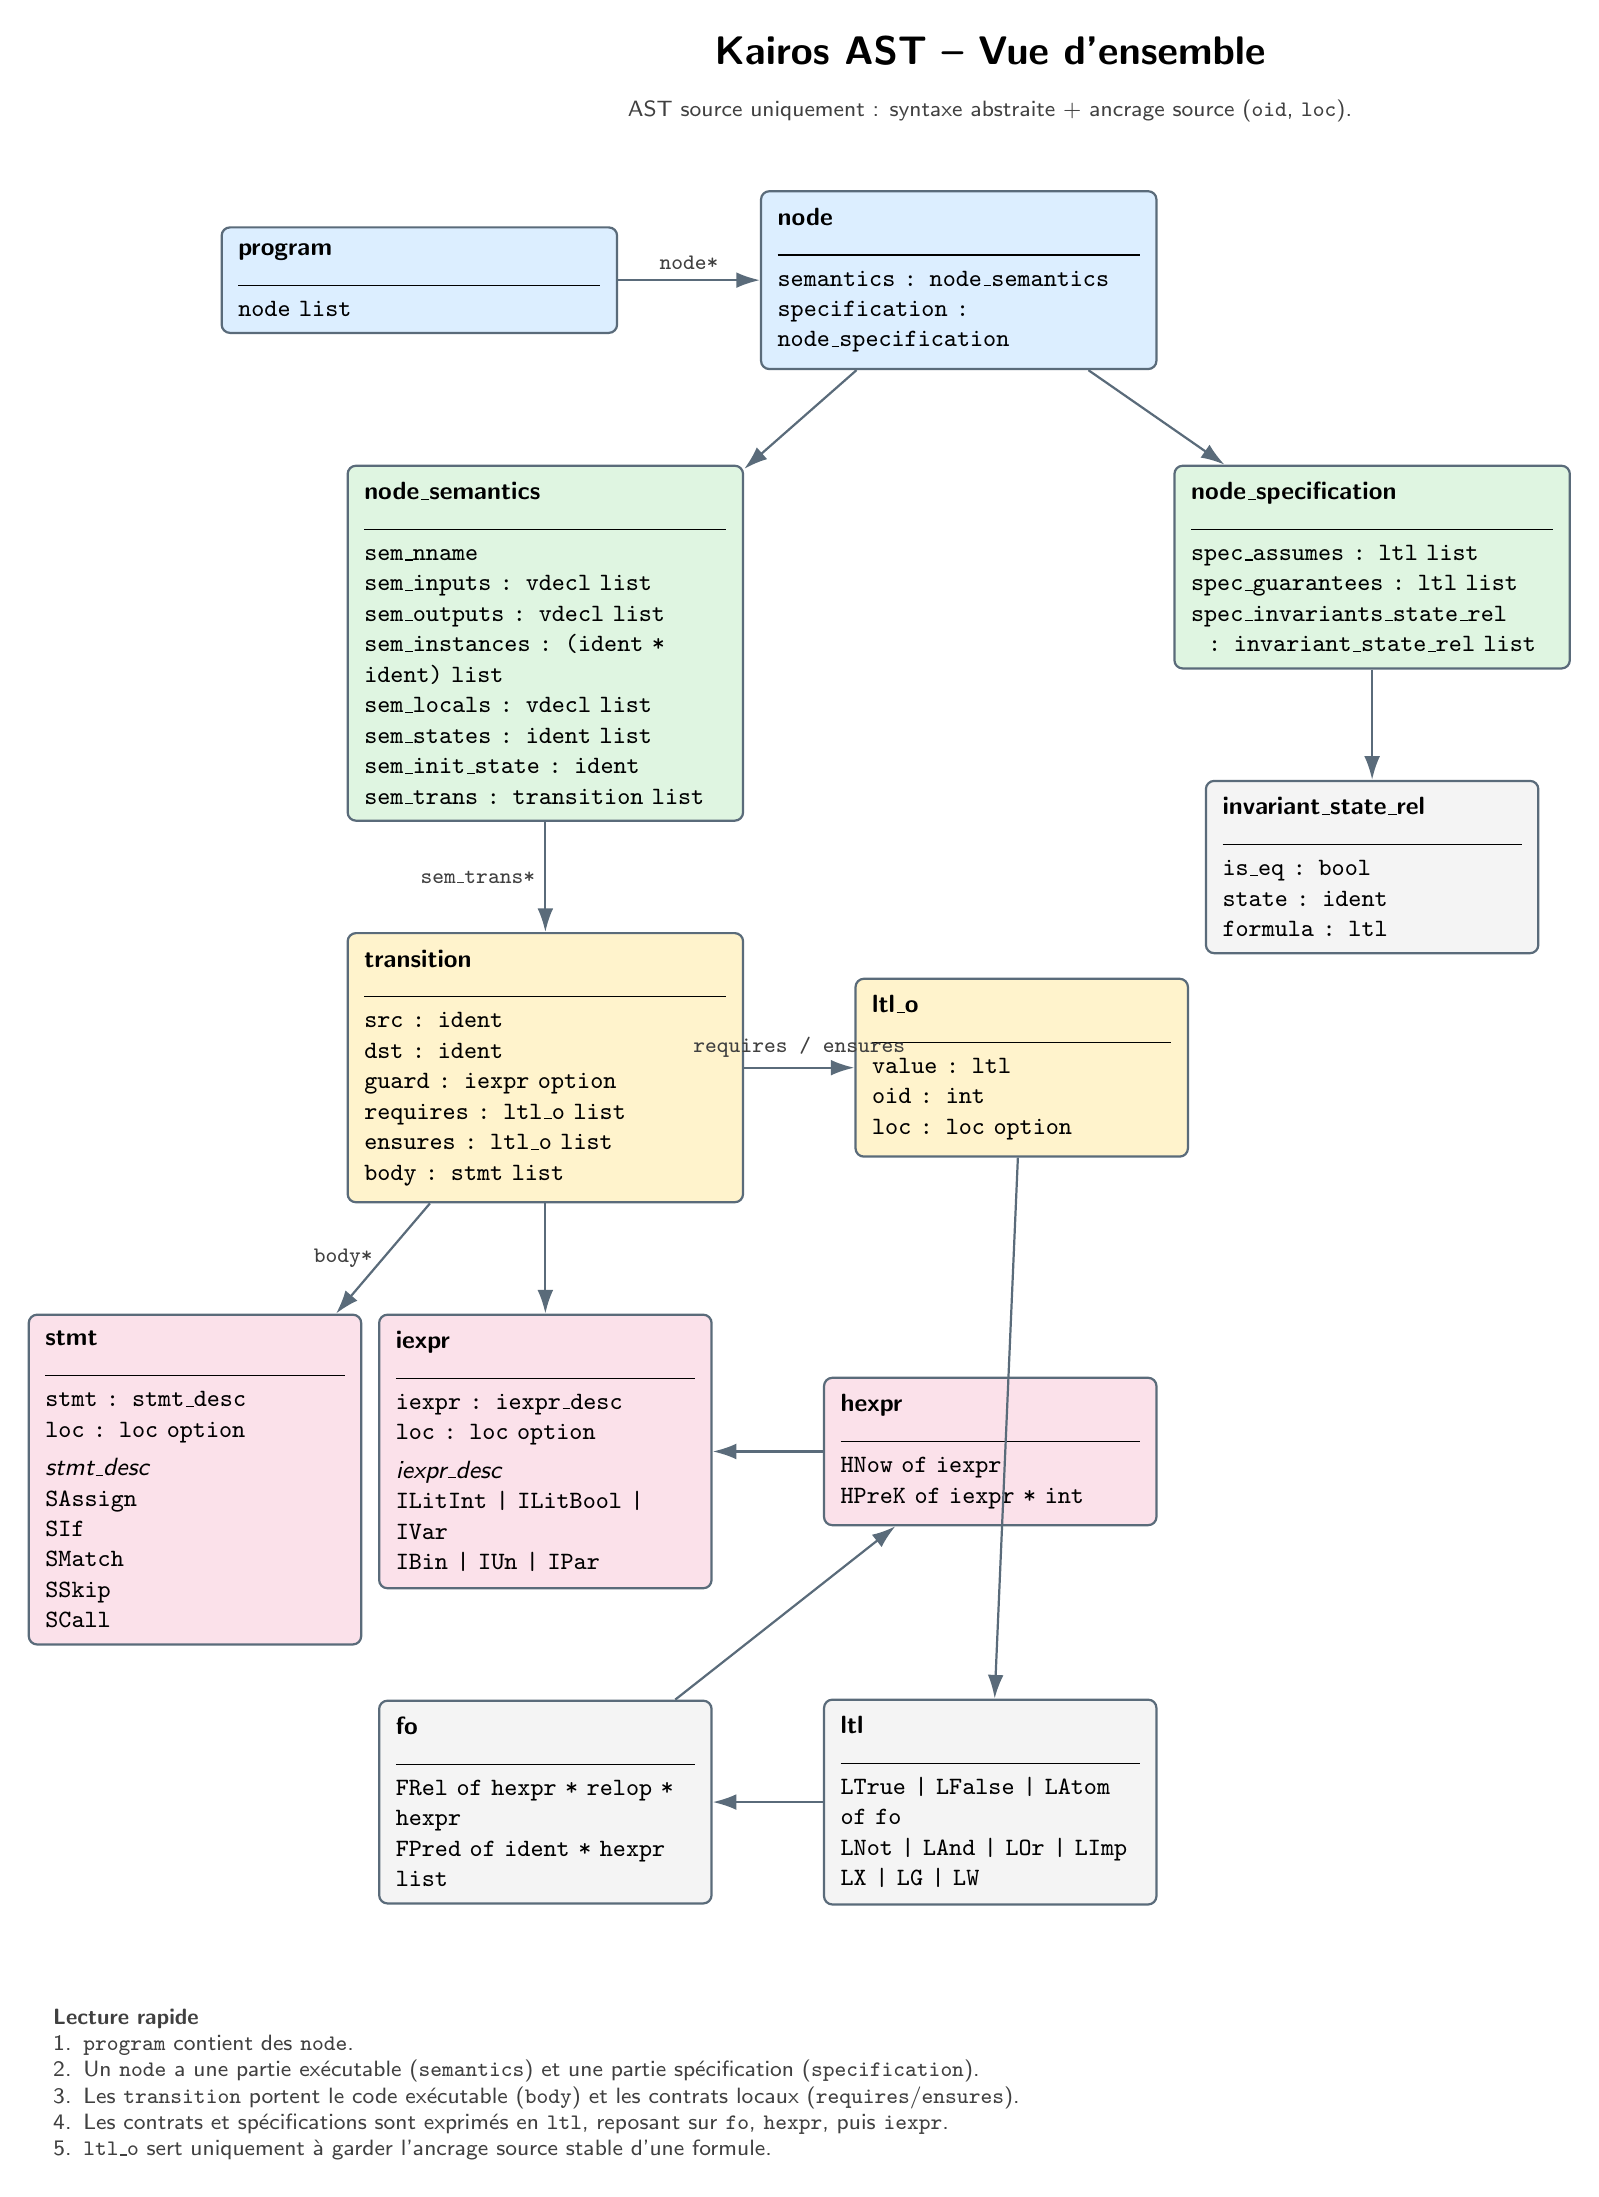
\begin{tikzpicture}[node distance=10mm and 12mm]

\node[title] (title) {Kairos AST -- Vue d'ensemble};
\node[note, below=2mm of title] (subtitle)
  {AST source uniquement : syntaxe abstraite + ancrage source (\texttt{oid}, \texttt{loc}).};

\node[box, fill=astblue, below left=12mm and 0mm of subtitle] (program) {
  \textbf{program}\\
  \rule{\linewidth}{0.4pt}\\
  \texttt{node list}
};

\node[box, fill=astblue, right=18mm of program] (node) {
  \textbf{node}\\
  \rule{\linewidth}{0.4pt}\\
  \texttt{semantics : node\_semantics}\\
  \texttt{specification : node\_specification}
};

\node[box, fill=astgreen, below left=12mm and 2mm of node] (semantics) {
  \textbf{node\_semantics}\\
  \rule{\linewidth}{0.4pt}\\
  \texttt{sem\_nname}\\
  \texttt{sem\_inputs : vdecl list}\\
  \texttt{sem\_outputs : vdecl list}\\
  \texttt{sem\_instances : (ident * ident) list}\\
  \texttt{sem\_locals : vdecl list}\\
  \texttt{sem\_states : ident list}\\
  \texttt{sem\_init\_state : ident}\\
  \texttt{sem\_trans : transition list}
};

\node[box, fill=astgreen, below right=12mm and 2mm of node] (specification) {
  \textbf{node\_specification}\\
  \rule{\linewidth}{0.4pt}\\
  \texttt{spec\_assumes : ltl list}\\
  \texttt{spec\_guarantees : ltl list}\\
  \texttt{spec\_invariants\_state\_rel}\\
  \texttt{\ \ : invariant\_state\_rel list}
};

\node[box, fill=astyellow, below=14mm of semantics] (transition) {
  \textbf{transition}\\
  \rule{\linewidth}{0.4pt}\\
  \texttt{src : ident}\\
  \texttt{dst : ident}\\
  \texttt{guard : iexpr option}\\
  \texttt{requires : ltl\_o list}\\
  \texttt{ensures : ltl\_o list}\\
  \texttt{body : stmt list}
};

\node[smallbox, fill=astyellow, right=14mm of transition] (ltlo) {
  \textbf{ltl\_o}\\
  \rule{\linewidth}{0.4pt}\\
  \texttt{value : ltl}\\
  \texttt{oid : int}\\
  \texttt{loc : loc option}
};

\node[smallbox, fill=astpink, below left=14mm and -2mm of transition] (stmt) {
  \textbf{stmt}\\
  \rule{\linewidth}{0.4pt}\\
  \texttt{stmt : stmt\_desc}\\
  \texttt{loc : loc option}\\[1mm]
  \textit{stmt\_desc}\\
  \texttt{SAssign}\\
  \texttt{SIf}\\
  \texttt{SMatch}\\
  \texttt{SSkip}\\
  \texttt{SCall}
};

\node[smallbox, fill=astpink, below=14mm of transition] (iexpr) {
  \textbf{iexpr}\\
  \rule{\linewidth}{0.4pt}\\
  \texttt{iexpr : iexpr\_desc}\\
  \texttt{loc : loc option}\\[1mm]
  \textit{iexpr\_desc}\\
  \texttt{ILitInt | ILitBool | IVar}\\
  \texttt{IBin | IUn | IPar}
};

\node[smallbox, fill=astpink, right=14mm of iexpr] (hexpr) {
  \textbf{hexpr}\\
  \rule{\linewidth}{0.4pt}\\
  \texttt{HNow of iexpr}\\
  \texttt{HPreK of iexpr * int}
};

\node[smallbox, fill=astgray, below=14mm of iexpr] (fo) {
  \textbf{fo}\\
  \rule{\linewidth}{0.4pt}\\
  \texttt{FRel of hexpr * relop * hexpr}\\
  \texttt{FPred of ident * hexpr list}
};

\node[smallbox, fill=astgray, right=14mm of fo] (ltl) {
  \textbf{ltl}\\
  \rule{\linewidth}{0.4pt}\\
  \texttt{LTrue | LFalse | LAtom of fo}\\
  \texttt{LNot | LAnd | LOr | LImp}\\
  \texttt{LX | LG | LW}
};

\node[smallbox, fill=astgray, below=14mm of specification] (inv) {
  \textbf{invariant\_state\_rel}\\
  \rule{\linewidth}{0.4pt}\\
  \texttt{is\_eq : bool}\\
  \texttt{state : ident}\\
  \texttt{formula : ltl}
};

\draw[arrow] (program) -- node[midway, above, note] {\texttt{node*}} (node);
\draw[arrow] (node) -- (semantics);
\draw[arrow] (node) -- (specification);
\draw[arrow] (semantics) -- node[midway, left, note] {\texttt{sem\_trans*}} (transition);
\draw[arrow] (transition) -- node[midway, above, note] {\texttt{requires / ensures}} (ltlo);
\draw[arrow] (transition) -- node[midway, left, note] {\texttt{body*}} (stmt);
\draw[arrow] (transition) -- (iexpr);
\draw[arrow] (ltlo) -- (ltl);
\draw[arrow] (specification) -- (inv);
\draw[arrow] (ltl) -- (fo);
\draw[arrow] (fo) -- (hexpr);
\draw[arrow] (hexpr) -- (iexpr);

\node[note, below=12mm of fo, text width=12.5cm] (legend) {
  \textbf{Lecture rapide}\\
  1. \texttt{program} contient des \texttt{node}.\\
  2. Un \texttt{node} a une partie exécutable (\texttt{semantics}) et une partie spécification (\texttt{specification}).\\
  3. Les \texttt{transition} portent le code exécutable (\texttt{body}) et les contrats locaux (\texttt{requires}/\texttt{ensures}).\\
  4. Les contrats et spécifications sont exprimés en \texttt{ltl}, reposant sur \texttt{fo}, \texttt{hexpr}, puis \texttt{iexpr}.\\
  5. \texttt{ltl\_o} sert uniquement à garder l'ancrage source stable d'une formule.
};

\end{tikzpicture}
\end{document}
